
% to choose your degree
% please un-comment just one of the following
\documentclass[bsc,frontabs,twoside,singlespacing,parskip,deptreport]{infthesis}     % for BSc, BEng etc.
% \documentclass[minf,frontabs,twoside,singlespacing,parskip,deptreport]{infthesis}  % for MInf

\usepackage{graphicx}

\begin{document}

\title{Sensing Spaces: Personal Exposure to Air Pollution with Different Modes of Transport and Urban Environments Using Wearable Sensors}

\author{Mihai Visuian}

% to choose your course
% please un-comment just one of the following
%\course{Artificial Intelligence and Computer Science}
%\course{Artificial Intelligence and Software Engineering}
%\course{Artificial Intelligence and Mathematics}
%\course{Artificial Intelligence and Psychology }   
%\course{Artificial Intelligence with Psychology }   
%\course{Linguistics and Artificial Intelligence}    
\course{Computer Science}
%\course{Software Engineering}
%\course{Computer Science and Electronics}    
%\course{Electronics and Software Engineering}    
%\course{Computer Science and Management Science}    
%\course{Computer Science and Mathematics}
%\course{Computer Science and Physics}  
%\course{Computer Science and Statistics}    

% to choose your report type
% please un-comment just one of the following
%\project{Undergraduate Dissertation} % CS&E, E&SE, AI&L
%\project{Undergraduate Thesis} % AI%Psy
\project{4th Year Project Report}

\date{\today}

\abstract{
This is an example of {\tt infthesis} style.
The file {\tt skeleton.tex} generates this document and can be 
used to get a ``skeleton'' for your thesis.
The abstract should summarise your report and fit in the space on the 
first page.
%
You may, of course, use any other software to write your report,
as long as you follow the same style. That means: producing a title
page as given here, and including a table of contents and bibliography.
}

\maketitle

\section*{Acknowledgements}

I would like to thank my supervisor, professor D K Arvind for his main support in helping me work thoroughly on a project of such high complexity and importance in the real world. I would also like to thank him for his valuable advice and guidance.

Furthermore, I would like to thank Andrew Bates for his support in providing equipment and helping with maintenance of sensors and servers.

\tableofcontents

%\pagenumbering{arabic}


\chapter{Introduction}

\section{Motivation}

Air pollution in large urban environments is a controversial topic nowadays and pollution sources, as well as distribution and effect on human health have been widely studied. Particulate matter (PM) represents the sum of all solid particles and liquid droplets of small sizes that are suspended in the air. It has been discovered that exposure to such particles of size less than 10 microns can be hazardous for the human body and it has been associated with increased mortality rates in areas labelled as highly polluted \cite{Dockery1994}.

Air quality is mostly measured through stationary Air Quality Monitoring Stations (AQMS). They measure air quality at a fixed location on a certain radius with high precision. Data collected from such networks of stations distributed strategically within urban environments is used to determine exposure to pollutants and is used for checking if a specific area meets requirements set by legislation. One drawback of this approach is that monitoring a large fixed region through a stationary sensor would not always suffice to obtain accurate information about air quality and pollution sources, as parameters vary from a corner of the region to another and other external factors such as wind speed and terrain type affect the results.

One approach to solve this issue and obtain more accurate data from the environment would be to deploy low-cost mobile sensors on people, such as drivers, pedestrians and cyclists in order to obtain a more precise spatial representation of the air quality. However, these sensors have to be calibrated in correlation with the Air Quality Monitoring Stations to ensure high precision of the information gathered.

\section{Objectives}

This project mainly focuses on Mobile Exposure Monitors (MEM) developed by the Centre for Speckled Computing. These wearable devices are equipped with sensors measuring humidity, temperature and particulate matter. Data is transmitted to an Android device via Bluetooth Low Energy. The project presents several study methods for detecting urban environments and personal exposure with different means of transport, based on air quality data collected with the wearable sensors. The objectives of the project are:

\begin{itemize}
\item Collect data at specific times on a daily basis and on a fixed route.
\item Perform analysis on data gathered for various modes of transport and urban environments and research machine learning techniques to detect personal exposure on a specific mode of transport or urban environment based on temperature, humidity and particulate matter attributes.
\item Build a data visualization tool for a more accurate spatial representation of data gathered and results obtained after applying statistical and machine learning methods.
\item Validate measurements of sensors against a more accurate Air Quality Monitoring Station in Edinburgh.
\end{itemize}

\section{Literature Review}

There are past studies concerning exposure of cyclists to air pollution and traffic noise in central neighbourhoods of Montreal \cite{Apparicio201663}. Despite it is known that cycling in urban areas would have beneficial effects on people's health, it is associated with potential health risks due to long time exposure to polluted air and traffic noise. The focus of this study was to analyse exposure of cyclists to air pollution and traffic noise and detect the impact on exposure of local factors such as weather conditions and the type of roads. A number of 85 bicycle trips were analysed, totalling 422 km of travel. The results revealed a weak negative correlation between noise and air pollution (NO$_2$) measures of exposure.

A study \cite{Dirks2012} done in Auckland, New Zealand, examined personal exposure to air pollution, namely carbon monoxide (CO) for several modes of transport, using Langan T15n \cite{Langan} portable carbon monoxide monitors. Participants were constrained to travel at specific peak traffic times between designated start and end points. Results suggest that lowest exposure to CO particles are experienced by train commuters, while motorcyclists were exposed to significantly higher average concentrations. Furthermore, travel by bus on a dedicated route proved to be more effective than travel by car on a congested motorway. Also, average exposure of cyclists and pedestrians proved to be similar to bus and car commuters. However, when increased physical activity that implies higher volumes of air breathed, along with increased commuting time were taken into account, air pollution dosage became much higher than for the motorised means of transport.

Most research regarding particulate matter has been performed in terms of values of PM2.5 and PM10, namely measurements of mass particulates with lower dimensions than 2.5 and 10 microns. A study \cite{Cho2008} is concerned about the relationship between mortality rate and particulate matter measured in Seoul, South Korea by an Optical Particulate Counter (OPC) and a national monitoring station. Particulate matter (PM2.5 and PM10) and particle counts from 0.3 to 25 microns were measured. The results concerning particle counts were associated with a 5.73\% and 5.82\% in mortality caused by respiratory diseases.

\section{Method}

Data collection has been performed in several phases, using a monitoring device worn around the chest, measuring particulate matter (PM1, PM2.5 and PM10 values along with particle counts of different sizes), as well as temperature and humidity. The sensor communicates with an Android device via Bluetooth to which the data gathered is sent. First, data was gathered on Nicholson Street while using a taxi to Calton Hill during midday. Then, data was gathered while walking on the same route, at the same time of the day, in order to perform the first classification analysis between different means of transport (walking as opposed to cars). For further investigation of personal exposure with different modes of transport, another set of data collected was obtained from a train trip from Edinburgh to London King's Cross, including a bus trip to Edinburgh Waverley, as well as walking trips in Edinburgh, London and London Underground.

Data analysis has been performed using Python and Jupyter Notebooks. First, the raw data was labelled accordingly in terms of the mean of transport used at each point in time. Secondly, the raw data was checked for any outliers existing in all the values of interest. After removing all irrelevant outliers, several machine learning classifiers have been used on PM data, along with temperature and humidity, in order to perform a classification of means of transport used during personal exposure experiments.

As far as personal exposure with different urban environments is concerned, a data collection schedule has been organised on a route in Edinburgh, including Nicholson Street, Melville Drive, Middle Meadow Walk, Tollcross and Lauriston Place, so that all types of urban environments would be detected. More exactly, the same route was covered over a week at two different times of the day, first at midday, during lunchtime between 13:00 and 14:00 and then in the evening, between 17:00 and 18:00, when a traffic peak hour is most probable to occur.

As in the previous set of experiments, Jupyter Notebooks have been used for analysis of the dataset regarding different urban environments. In this case, unsupervised machine learning methods have been applied for classification of data, as ranges of PM values corresponding to each urban environment type vary from a region to another. Thus, K-means clustering was performed first on the coordinates of the dataset features, such that all samples would be grouped into compact clusters and the mean values of the PM related values would be computed for each cluster. Then, a second K-means clustering was applied to the mean values of the clusters obtained in the previous step in order to detect the different types of urban environments.

\section{Structure of the Report}

Chapter 2 reveals detailed information regarding equipments used in the data collection phase, as well as details about PM measurements obtained. Moreover, details about the modes of transport used and types of urban environments taken into consideration are presented.

Chapter 3 details the data collection phase. Then, it also introduces details about statistics and machine learning techniques used in the data analysis process. Moreover, it introduces a data visualization tool implemented from scratch to ease analysis of data collected. Details about this tool will be further discussed in the following chapter.

Chapter 4 details on the data visualization tool, focusing both on the purpose and the functionality of the tool. The application is formed of two main parts, namely the front-end dealing with the spatial representation of the data on a map and the back-end, which consists of an API making requests to the data collected which is stored in a database.

Chapter 5 presents the results obtained from the data analysis phase. First, a research regarding classification of pollution exposure with different modes of transport is done using various machine learning classifiers. Then, unsupervised data is used to detect several types of urban environments, which will be presented in detail in chapter 2.

Finally, chapter 6 presents the conclusions drawn from the results obtained from data analysis and described in detail in chapter 5. Moreover, potential improvements and further study areas regarding the main topic of the project worth exploring are described.

\chapter{State of the Art}

\section{Mobile Exposure Monitor}

The Mobile Exposure Monitor (MEM) is a wearable device developed with the purpose of quality of environment measurement by the Centre for Speckled Computing. It is equipped with sensors measuring particulate matter counts and mass (Alphasense OPC-N1), as well as temperature and humidity (Sensirion SHT-75). The device transmits sensor readings via Bluetooth Low Energy (BLE) technology to a smart phone or tablet.

\section{Alphasense Optical Particulate Counter}

\section{Urban Environments}

As far as urban environments detection is concerned, five different types of urban environments are taken into consideration in terms of the average values of the bin counts:

\begin{itemize}
\item park paths
\item pedestrian areas
\item quiet roads
\item medium traffic areas
\item crowded / high traffic areas
\end{itemize}

\section{Personal Exposure with Modes of Transport}

In order to study personal exposure in all cases, six different exposure situations corresponding to six different modes of transport used have been taken into consideration especially during the data collection process:

\begin{itemize}
\item pedestrian data
\item car
\item train
\item bicycle
\item bus
\item subway (in London)
\end{itemize}

\chapter{Methodology}

\section{Data Collection Process}

During the project development, an annotated dataset with modes of transport used at each point was created for data analysis. Most of the data was collected in the first semester, more exactly during November and December. First data collection was performed during a train journey from Edinburgh to Manchester, on a route between several train stations for one hour.

Moreover, a major phase of data collection involving the analysis of different types of urban environments occurred between the 3rd and the 8th of December. More precisely, data capturing particulate matter counts had been collected using the MEM, by walking on a fixed route around meadows based on a daily schedule for a week (Figure \ref{fig:december_route}). The route was scanned twice a day, both during lunch time between 13:00 and 14:00 and in the afternoon between 17:30 and 18:30, so that the same path would be examined at different times of the day involving different intensities of the traffic.

\begin{figure}[h]
  \center
  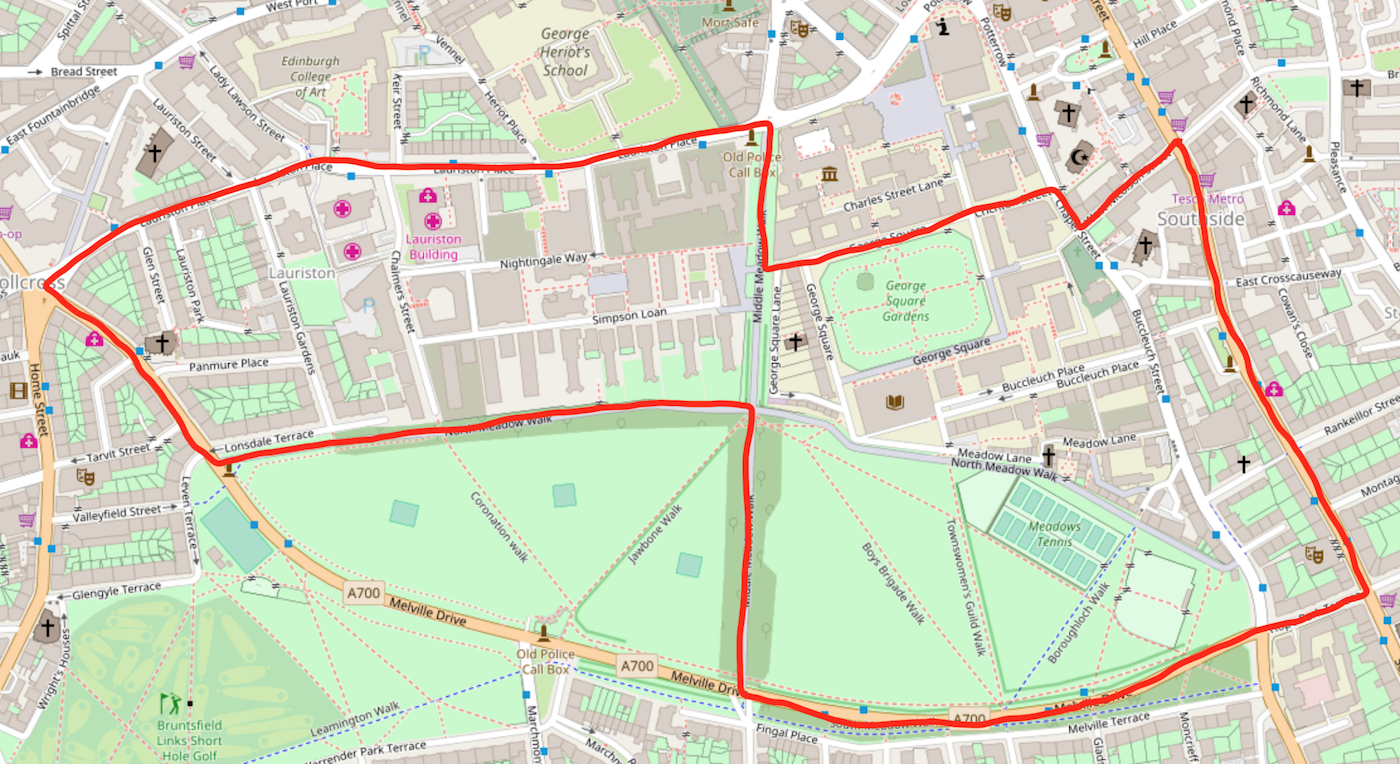
\includegraphics[width=\columnwidth]{december_route.png} 
  \caption{This map of Meadows region emphasises the route that was scanned while walking in December based on the schedule mentioned.}
  \label{fig:december_route}
\end{figure}

More data gathered and annotated with the purpose of studying personal exposure with different modes of transport has been obtained from \textbf{[NAME]} who commuted to work by car and wore the device for two consecutive days. He also used the sensors on a train journey to London and around the city centre, involving bus and subway transport.

Furthermore, Aart Meijer, an MSc student whose honours project involved air quality prediction using wearable sensors on cyclists collected data on a fixed route around Meadows when he was commuting to university every day by bicycle. A part of the dataset containing approximately 1000 data points has been extracted and compared to a new set of data points collected in the evening of the 26th of February 2018, during the snow storm, in order to analyse how different weather affects sensor readings of particulate matter.

\section{Unsupervised Learning for Urban Environments Study}

\subsection{K-means Clustering on Particulate Matter}

\subsection{Generalising Clustering Approach}

\section{Supervised Learning for Modes of Transport Classification}

\subsection{Models Comparison}

\section{Data Analysis}

\chapter{Implementation}

\section{Data Visualisation Tool}

\subsection{Front-end Interface}

\subsection{Back-end Server}

\chapter{Results}

\section{Detection of Urban Environments}

\section{Comparison of Personal Exposure with Different Modes of Transport}

\subsection{Generalisation of Classification Model}

\subsection{Bin Counts Normalisation}

\chapter{Conclusions}

\section{Concluding Remarks}

\section{Future Work}

% use the following and \cite{} as above if you use BibTeX
% otherwise generate bibtem entries

\bibliographystyle{plain}
\bibliography{mybibfile}

\end{document}
